\documentclass{article}
\author{Abdelmalek Fathi, Maamar Choukri\\
Laarbi Tebessi Tebessa University\\
Math and Computer Science Departement}
\title{Build a web site for representing international conferences}
\date{}
\usepackage{graphicx}
\graphicspath{ {./images/} }
\renewcommand*\contentsname{Table of Contents}

\begin{document}
	\maketitle
	\clearpage
	\tableofcontents
	\clearpage
	\section{Introduction}
	\paragraph{}
	National and international scientific conferences are an important event for universities and researchers from different parts of the world, so it is necessary to facilitate the process of publishing and accessing these conferences.
	\paragraph{}
	Among the proposed solutions, we find that one of them relies on creating a website for publishing conferences and requesting registration in them, where the person in charge of the conference (university or organization) publishes the necessary information about the conference such as its name, date, and participation price, if any, while any researcher or student can Knowing the request to participate in it, as he sends his research to the officials in charge of the conference and is waiting for it to be accepted by them.
	\paragraph{}
	And this is the project that we were assigned to do as a graduation project.
	\paragraph{}
	This article contains the following chapters:
	\begin{itemize}
		
		\item \textbf{Presentation of the project frameworks :}
		Chapter to figure out the problem and its solution in details.
		
		\item \textbf{Analysis and design \textit{(UML)} :}
		Chapter to introduce the \textit{UML} diagrams that we used to analysis the project and figure out his functions.
		
		\item \textbf{The implementation :}
		Chapter to view  the technologies that we used in making the site, and the implementation of our site (pictures from the website itself).
		
	\end{itemize}
	\clearpage
	\section{Presentation of the project frameworks}
	
	\clearpage
	\section{Analysis and design (UML)}
	We have utilized the following graphs: class, use cases and sequence diagram of each process in our website
	\subsection{Class Diagram}
	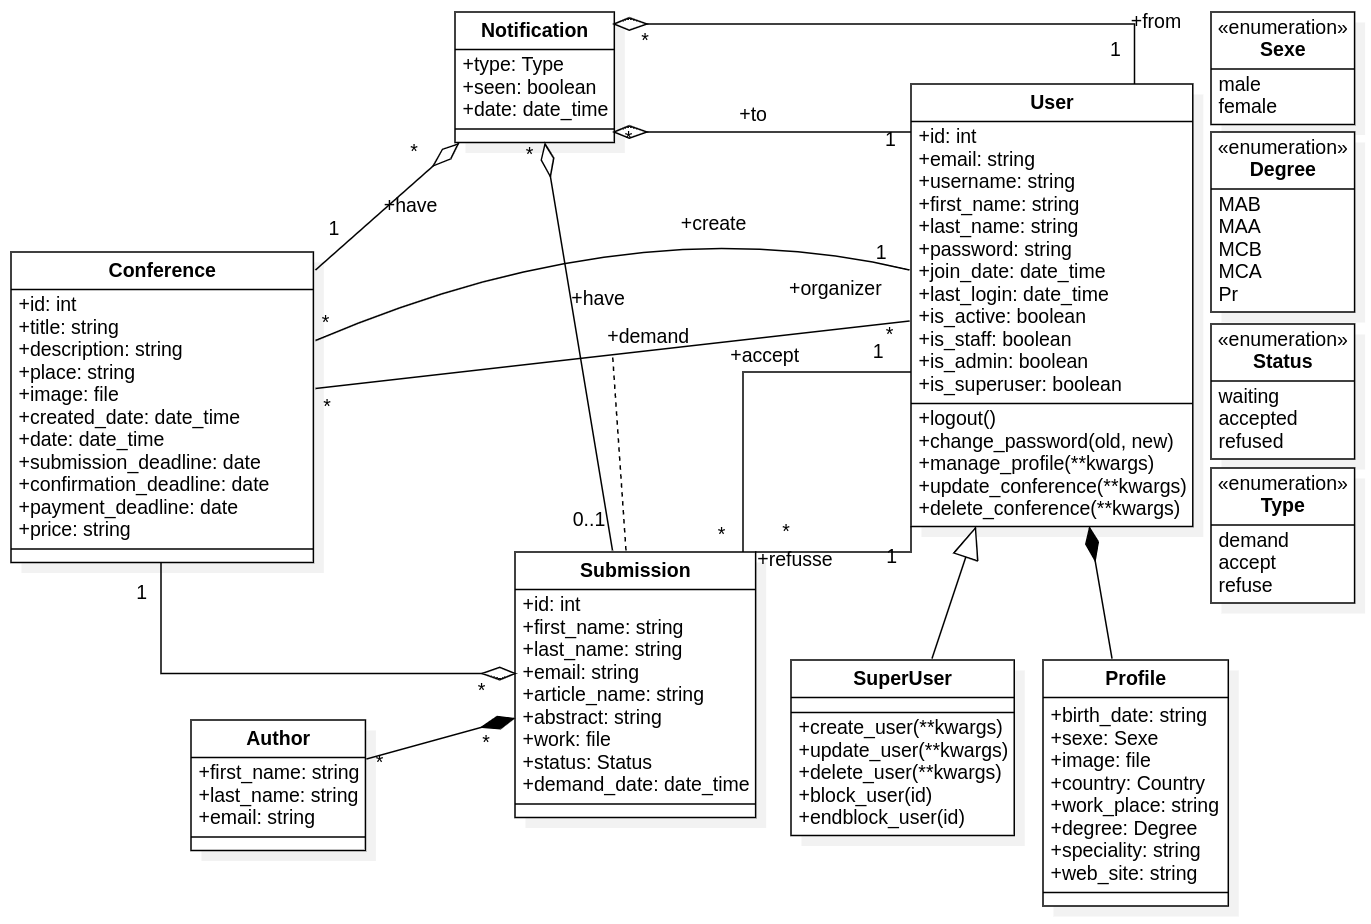
\includegraphics[scale=0.3]{diagrams/class.png}
	\subsection{User cases Diagram}
	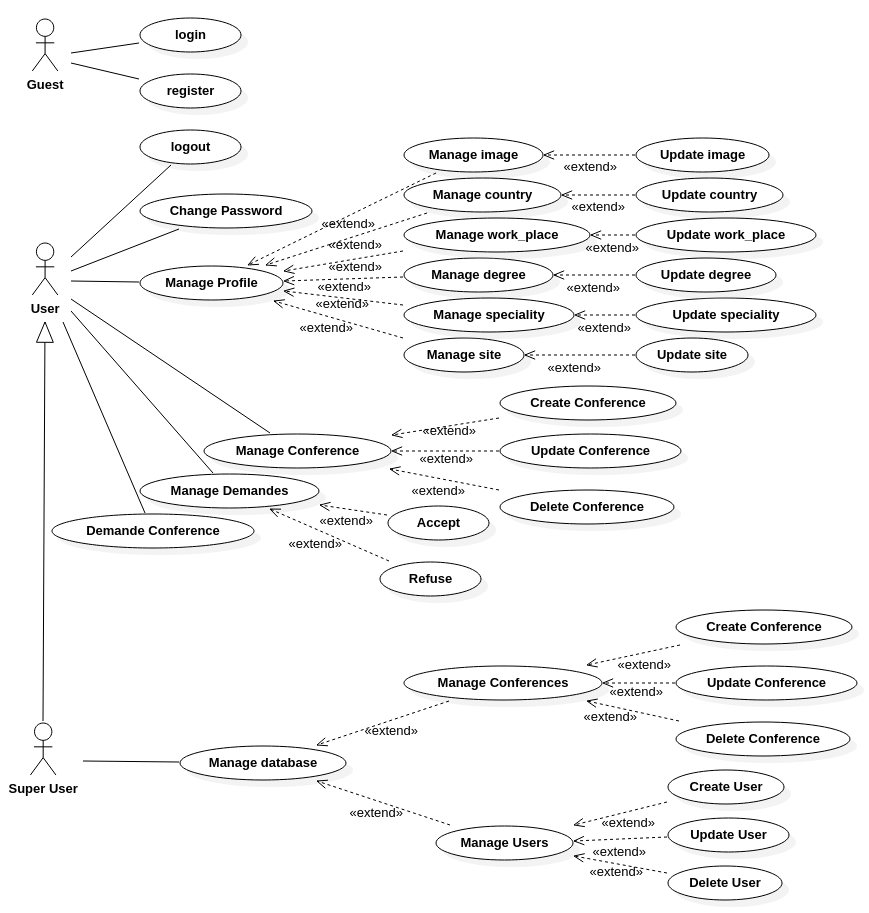
\includegraphics[scale=0.3]{diagrams/use_case.png}
	\subsection{Sequence Diagrams}
	\subsubsection{For add user}
	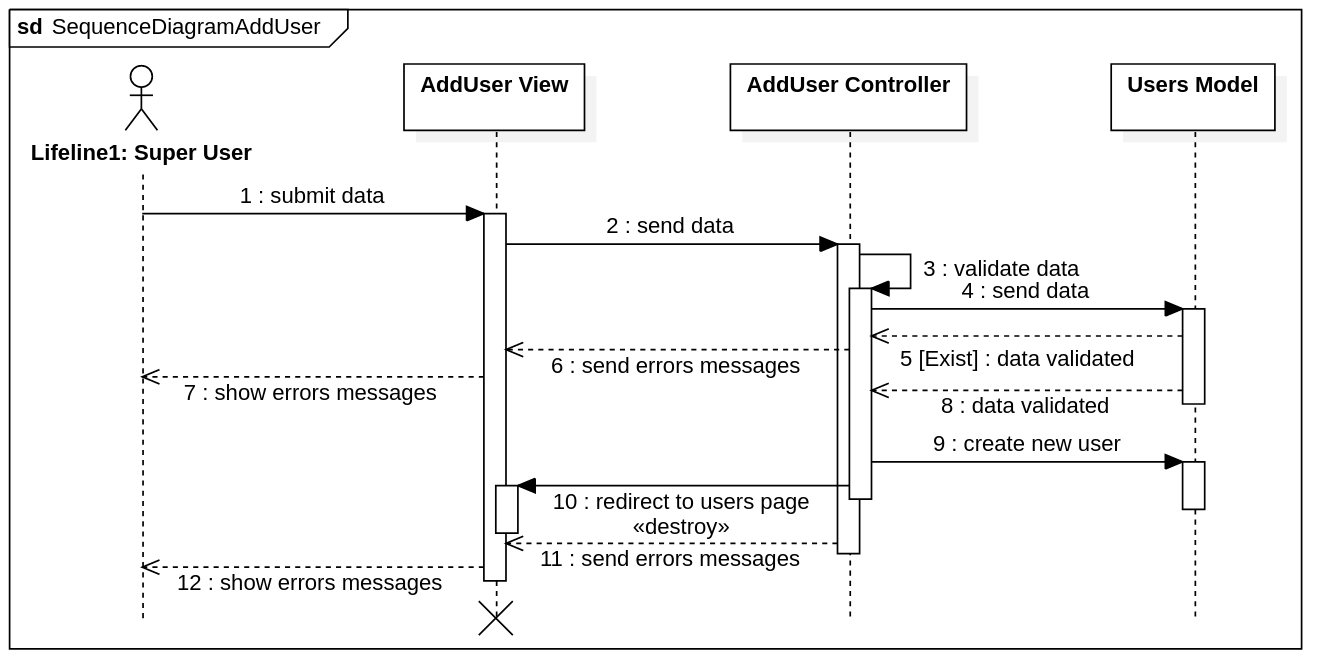
\includegraphics[scale=0.3]{diagrams/add_user_sequence.png}
	\subsubsection{For update user}
	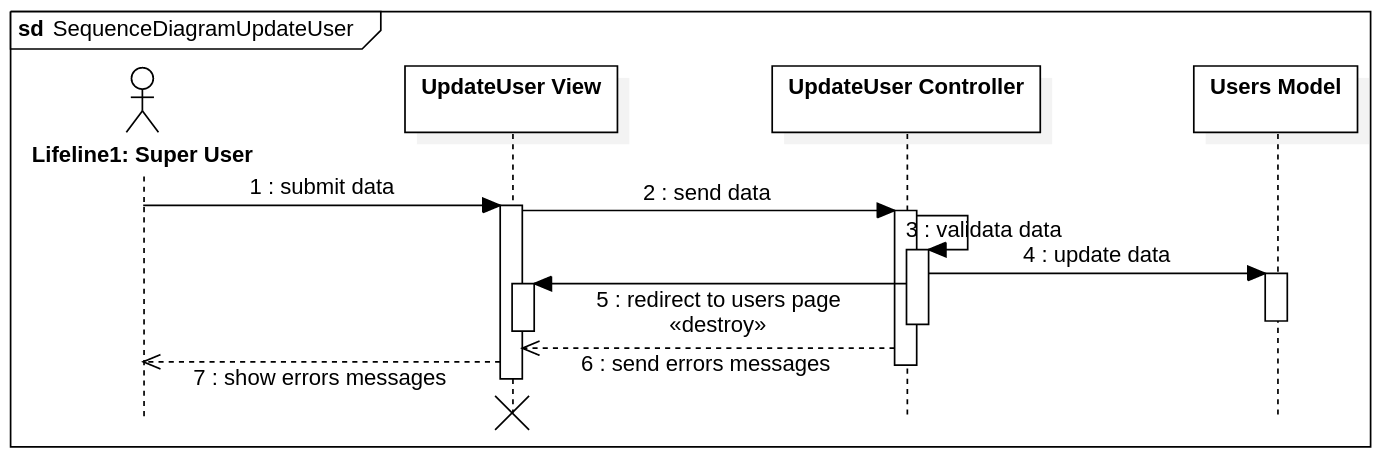
\includegraphics[scale=0.3]{diagrams/update_user_sequence.png}
	\subsubsection{For delete user}
	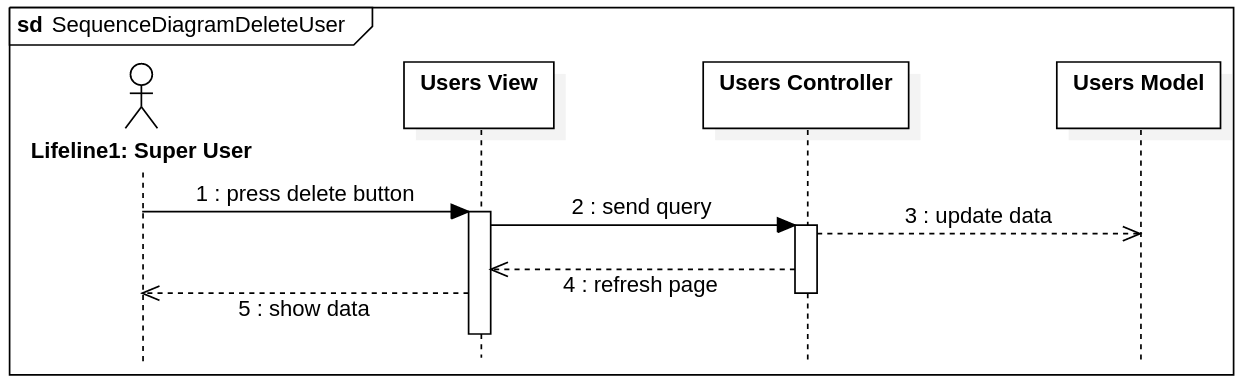
\includegraphics[scale=0.3]{diagrams/delete_user_sequence.png}
	\subsubsection{For block user}
	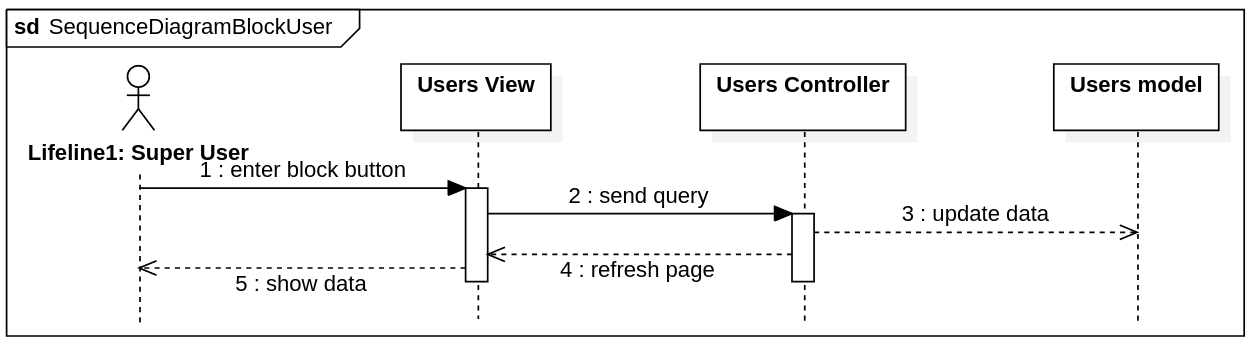
\includegraphics[scale=0.3]{diagrams/block_user_sequence.png}
	\subsubsection{For end block user}
	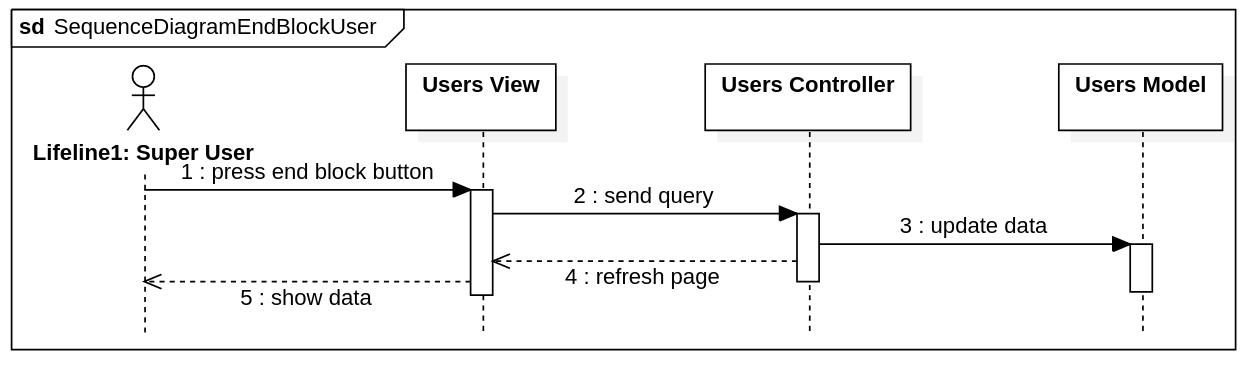
\includegraphics[scale=0.3]{diagrams/end_block_user_sequence.png}
	\subsubsection{For register}
	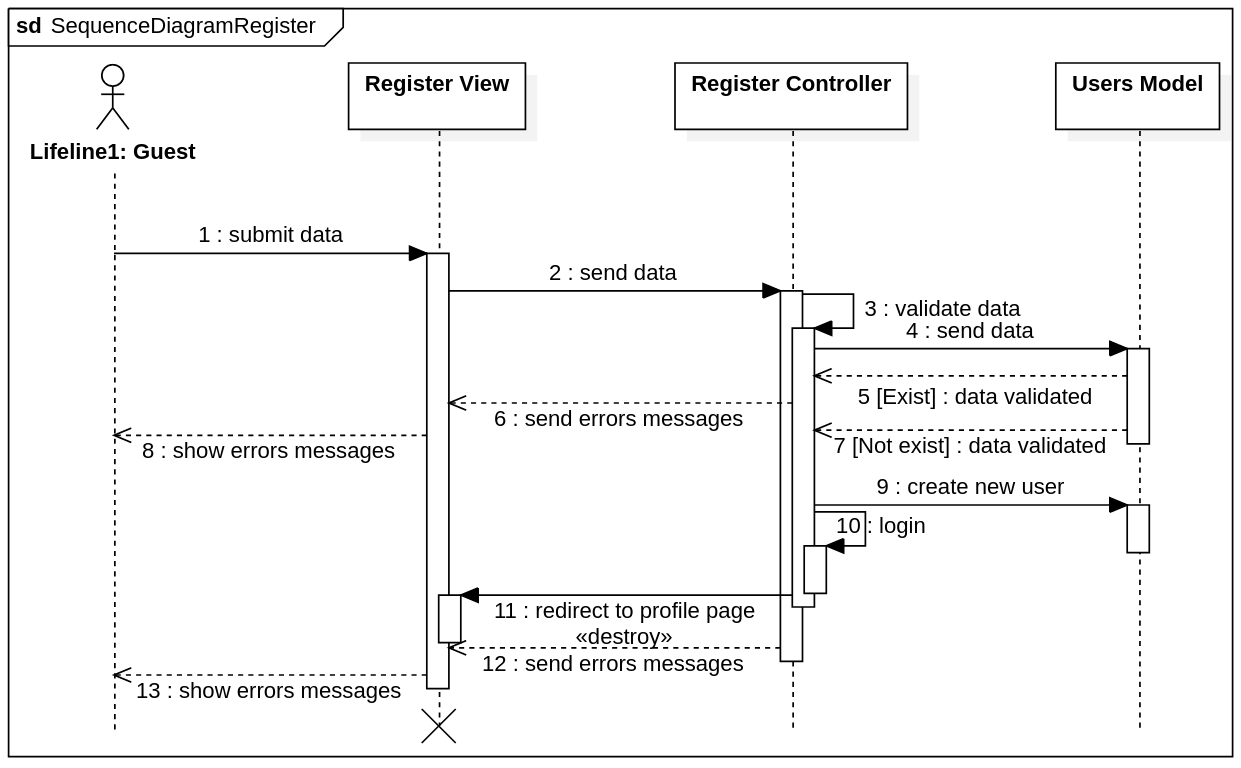
\includegraphics[scale=0.3]{diagrams/register_sequence.png}
	\subsubsection{For login}
	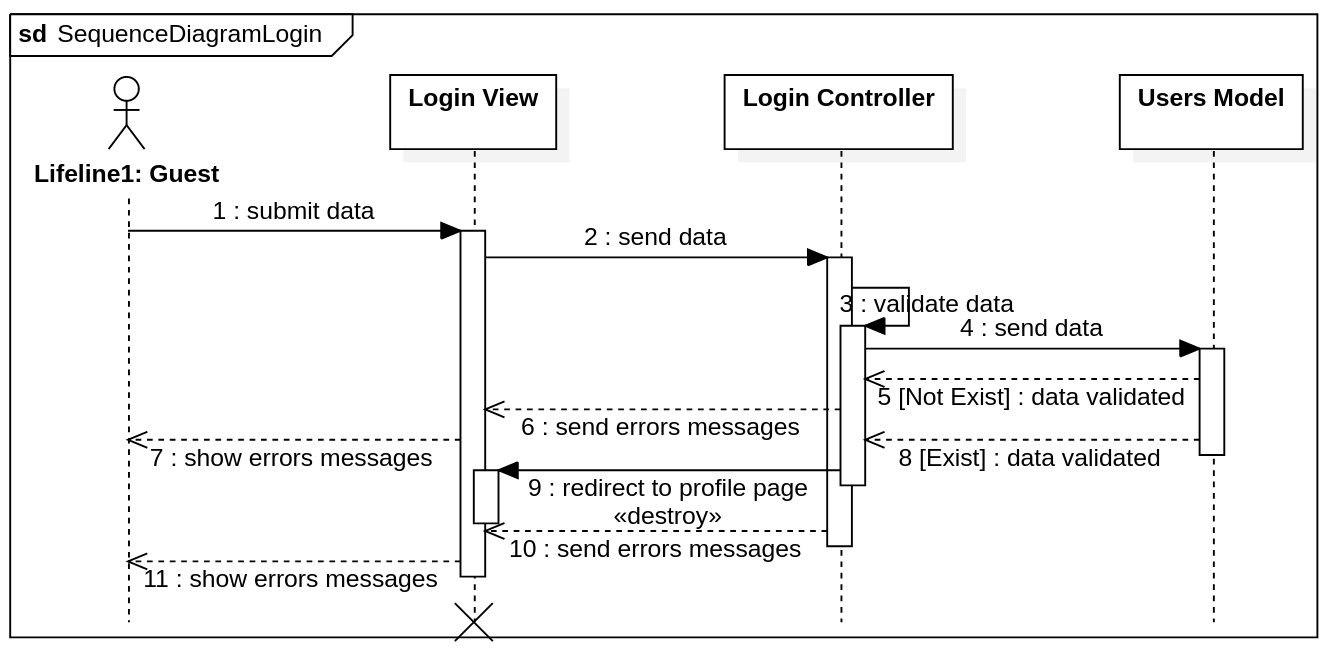
\includegraphics[scale=0.3]{diagrams/login_sequence.png}
	\clearpage
	\section{The implementation}
	\paragraph{}
	Any site is consist from front-end, back-end and database.
	\paragraph{}
	There are many technologies for each part of the website, but we choose the following technologies for our project:
	\subsection{For front-end}
	\subsubsection{HTML}
	\paragraph{}
	HTML (Hyper-Text Markup Language) is the standard mark-up language for documents designed to be displayed in a web browser. It can be assisted by technologies such as Cascading Style Sheets (CSS) and scripting languages such as JavaScript.
	\subsubsection{CSS}
	\subsubsection{JS}
	\subsubsection{JQuery}
	\subsubsection{Bootstrap}
	\subsubsection{Font Awesome}
	\subsection{For back-end}
	\subsubsection{Django Web Framework}
	\subsection{For database}
	\subsubsection{postgresql}
	\subsection{For web server}
	\subsubsection{gunicorn}
	\clearpage
	\section{Conclusion}
	
	\clearpage
%	\section{References}
	\begin{thebibliography}{9}
		\bibitem{HTML}
		https://en.wikipedia.org/wiki/HTML
	\end{thebibliography}
	
\end{document}
